\section{Diagrama Entidad Relación}
\subsection{Diagrama}

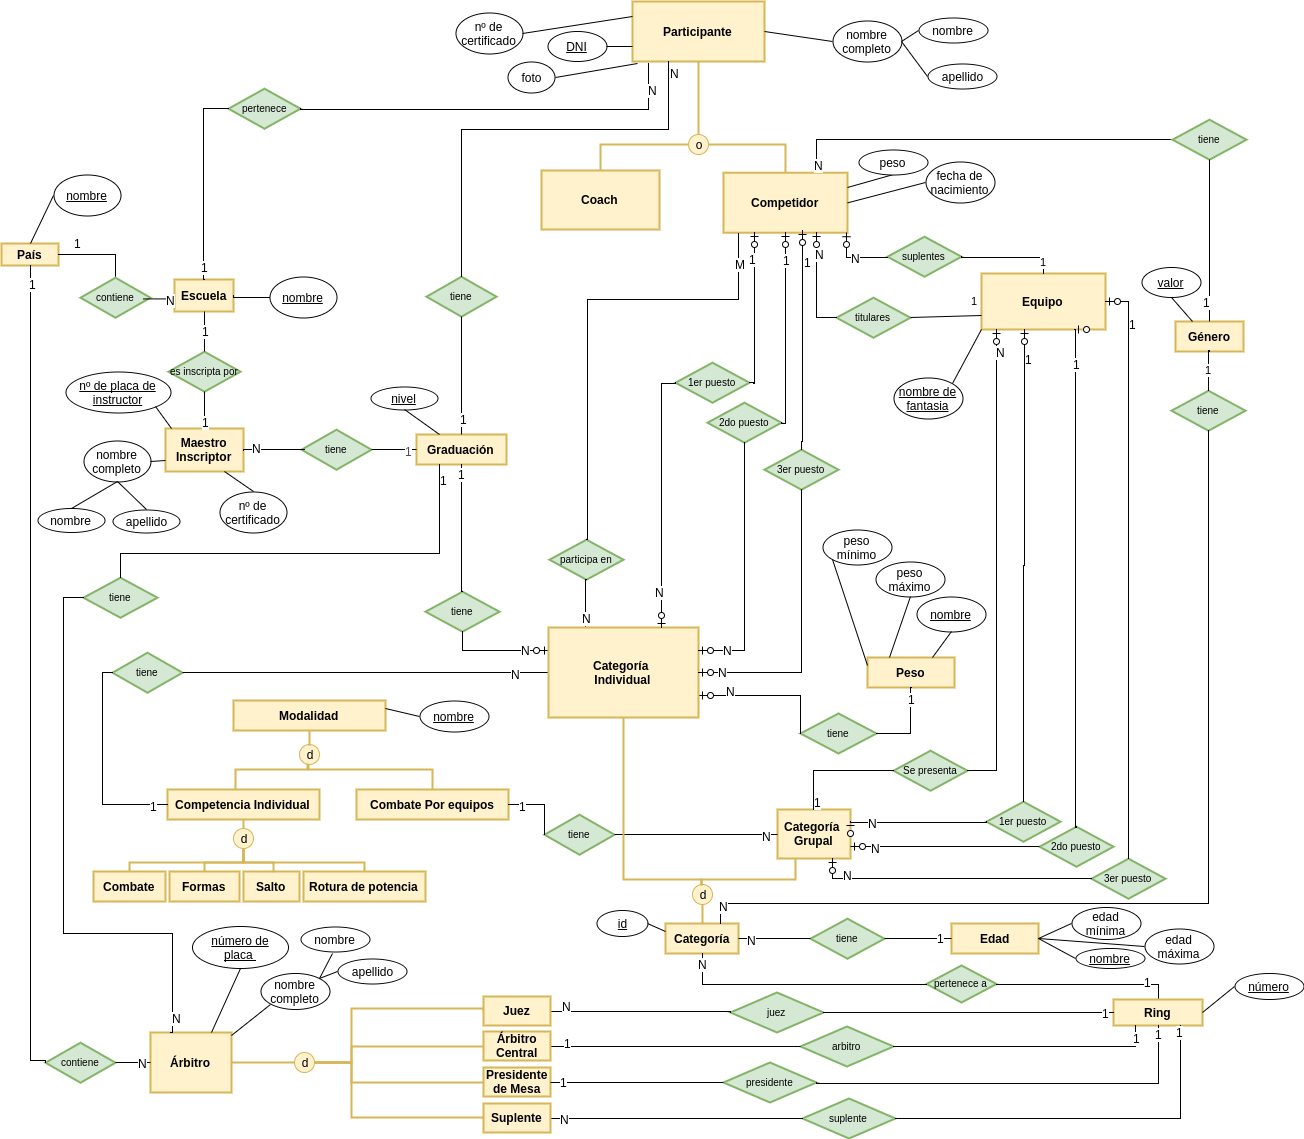
\includegraphics[scale=0.4]{der.png}

\newpage
\subsection{Restricciones}

\begin{enumerate}
\item Por escuela, la cantidad de coachs que presentan es $\lceil$ cantidad de alumnos / 5 $\rceil$.
\item Cada competidor, se puede presentar, a lo sumo, a una categoría de la misma modalidad.
\item Los competidores s\'olo se pueden presentar a categor\'ias que correspondan a sus caracter\'isticas (g\'enero, edad y/o peso).
\item Los equipos están integrados por 5 titulares y 3 suplentes.
\item Cada competidor, si pertenece a un equipo como Titular no debe pertenecer a ning\'un otro como Suplente.
\item Cada competidor, si pertenece a un equipo como Suplente no debe pertenecer a ning\'un otro como Titular.
\item Todos los competidores de un mismo equipo deben pertenecer a la misma escuela.
\item Todos los miembros de un mismo Equipo (titulares y suplentes) deben tener las caracter\'isticas que correspondan a la edad y al g\'enero de la categor\'ia que se presentan.
\item En el ring, los \'arbitros suplentes deben ser al menos 3 y los jueces son m\'as de 1.
\item La graduaci\'on de cada \'arbitro es superior a la graduaci\'on de la categor\'ia que arbitra.
\item El nivel de la graduacion se encuentra entre 1 y 6.
\item Un jugador s\'olo puede pertenecer a la terna de categor\'ias que participa.
\item Dada una categor\'ia individual: si ning\'un competidor se presenta, entonces no puede tener primer, segundo o tercer puesto.
\item Dada una categor\'ia individual: si s\'olo un competidor se presenta, entonces no puede tener segundo o tercer puesto.
\item Dada una categor\'ia individual: si se presentan dos competidores pasa que o bien no tiene ning\'un puesto o tiene primero y segundo.
\item Dada una categor\'ia individual: si se presentan tres competidores o m\'as pasa que o bien no tiene ning\'un puesto o tiene los tres.
\item Dada una categor\'ia individual, los tres primeros puestos son tres personas distintas.
\item Un equipo s\'olo puede pertenecer a la terna de las categor\'ias que participa.
\item Dada una categor\'ia grupal: si ning\'un equipo se presenta, entonces no debe tener primer, segundo o tercer puesto.
\item Dada una categor\'ia grupal: si s\'olo un equipo se presenta, entonces no puede tener segundo o tercer puesto.
\item Dada una categor\'ia grupal: si se presentan dos equipos pasa que o bien no tiene ning\'un puesto o tiene primero y segundo.
\item Dada una categor\'ia grupal: si se presentan tres equipos o m\'as pasa que o bien no tiene ning\'un puesto o tiene los tres.
\item Dada una categor\'ia grupal, los tres primeros puestos son tres equipos distintos.
\item La modalidad ``Combate'' es la \'unica que se clasifica por Peso.
\item La modalidad ``Formas'' es la \'unica que no se clasifica por Graduaci\'on, las dem\'as si.
\item Para todas las categor\'ias que presentan la misma modalidad, si se clasifican por edad, los rangos de edad son disjuntos.
\item Para todas las categor\'ias que presentan la misma modalidad, si se clasifican por peso, los rangos de peso son disjuntos.
\end{enumerate}
